\documentclass{standalone}
\begin{document}
	\subsection{Description}
	
	\textcolor{red}{As we have seen, the pipeline workflow involves three main steps.In this section I will discuss the general structure of the pipeline, more details about the actual implementation will be given in the next chapter.
	To perform the color quantization I've to found the characteristic color(centroids in the color space) of each tissue and use them for the actual segmentation, dividing the pipeline in two main steps.}

	
	\subsubsection*{Pre Processing and Lung Extraction}
	
	This preliminary step is performed before both training and labeling and involves the managing of the HU, the isolation of lung regions and the removal of the main bronchial structures.
	
	The registration of the HU on a common space is necessary to overcome the issues that may raise from the different padding values and multiplicative constant for HU computation (equation\,\ref{eq:HU}) used by the different manufacturer of the CT scans. The $k$ constant in the HU definition (equation\,\ref{eq:HU}) may change according to the scan manufacturer or scan model; moreover, during the scan acquisition, all the regions outside the CT tube aren't sampled, so to obtain a square $N\times N$ image for each slice some padding values are added, which different values according to the scan manufacturer. So a first registration was performed.
	
	
	Lung segmentation is a pivotal pre-processing step in many image analysis such as identification and classification of lung pathologies~\cite{ART:Johannes}. The lung isolation allow us to fund a mask for the lung regions, and thus excluding  all the body regions, the CT tube and the extra-lung organs like intestine and heart, avoiding the formation of false positives.
	
	Automatic lung segmentation algorithm are typically developed and tested on limited datasets and usually over a limited spectrum of visual variability by containing mainly cases without severe pathologies~\cite{ART:Johannes}. Rule based approach, like thresholding, region growing, ect, usually fails for CT sans of patients with severe Interstitial Lung Disease (ILD), as we can see in \figurename\,\ref{fig:UNetVSThr}. To achieve the lung segmentation I've used a pre-trained U-Net~\cite{ART:Johannes}~\cite{REP:lungmask}. 
	\begin{figure}[h!]
		\centering
		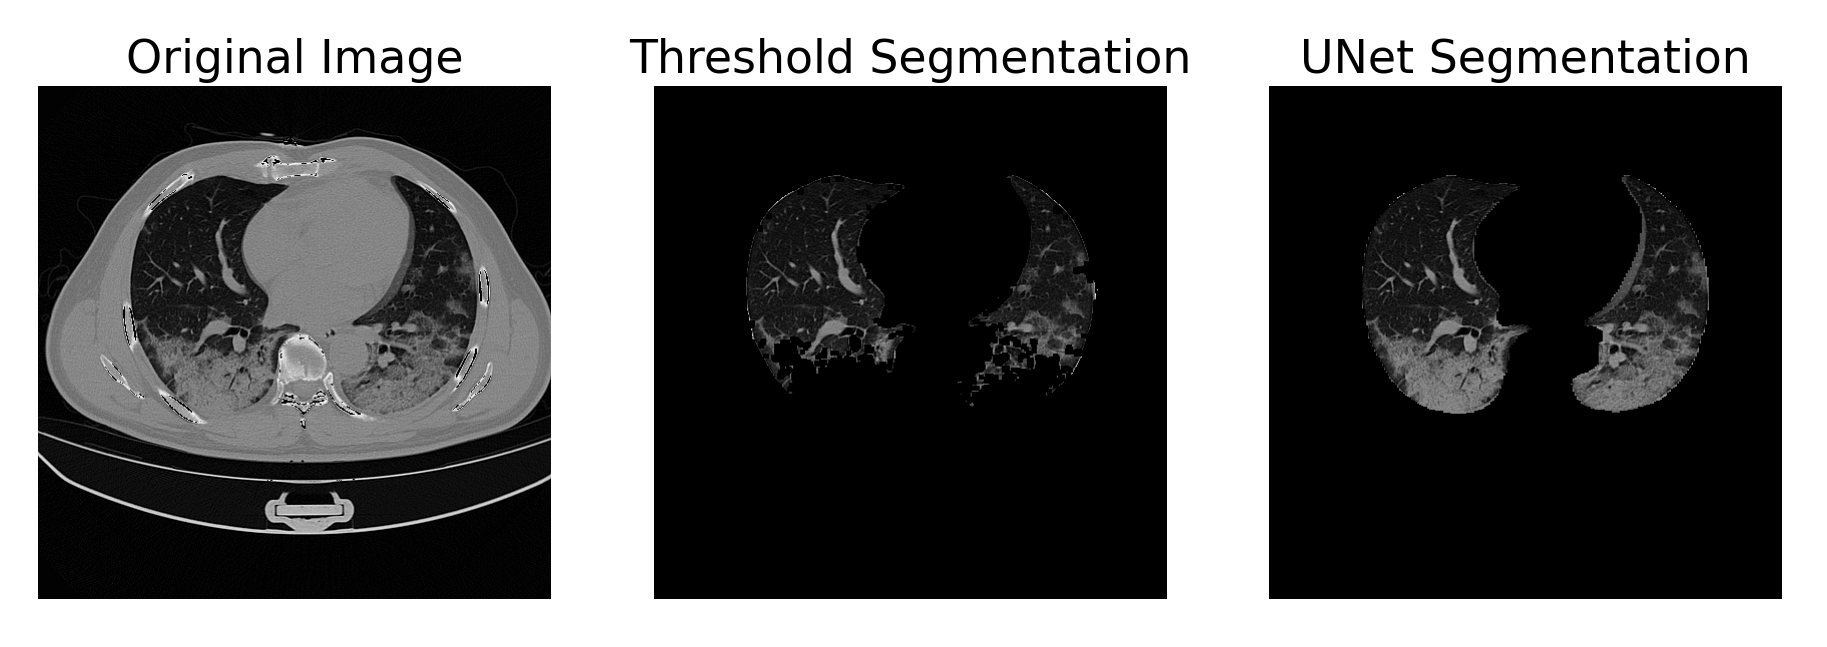
\includegraphics[scale=.5]{UNetVSThr.png}
		\caption{From left to right the original CT scan of a patient with severe ILD, the lung segmented by threshold and it's connected components, and lung segmentation achieved by the pre-trained U-Net. We can clearly see the missing areas in the first segmentation, correctly identified in the U-Net one.}\label{fig:UNetVSThr}
		
	\end{figure}
	
	This kind of segmentation includes in the lung region also motion artifacts and bronchial structures, which we will see are the principal causes of false positives. To achieve a better segmentation a refinement process is performed, which aims to remove the main bronchial structures form the selected lung regions. 
	
	Bronchi have an elongated shape respect to the other structure which usually are rounded: the basic Idea was to use this kind of information. In order to perform this task, I have  computed the covariant matrix of the derivative in a neighborhood and the corresponding eigenvalues. If a particular regions has an elongated shape, one of the eigenvalues (corresponding to the eigenvector in the direction of the structure) will have an higher value, otherwise both eigenvalues have a lower value. So we have applied this filter on each slice of the scans and took the maximum eigenvalues. 
	\begin{figure}[h!]
		\centering
		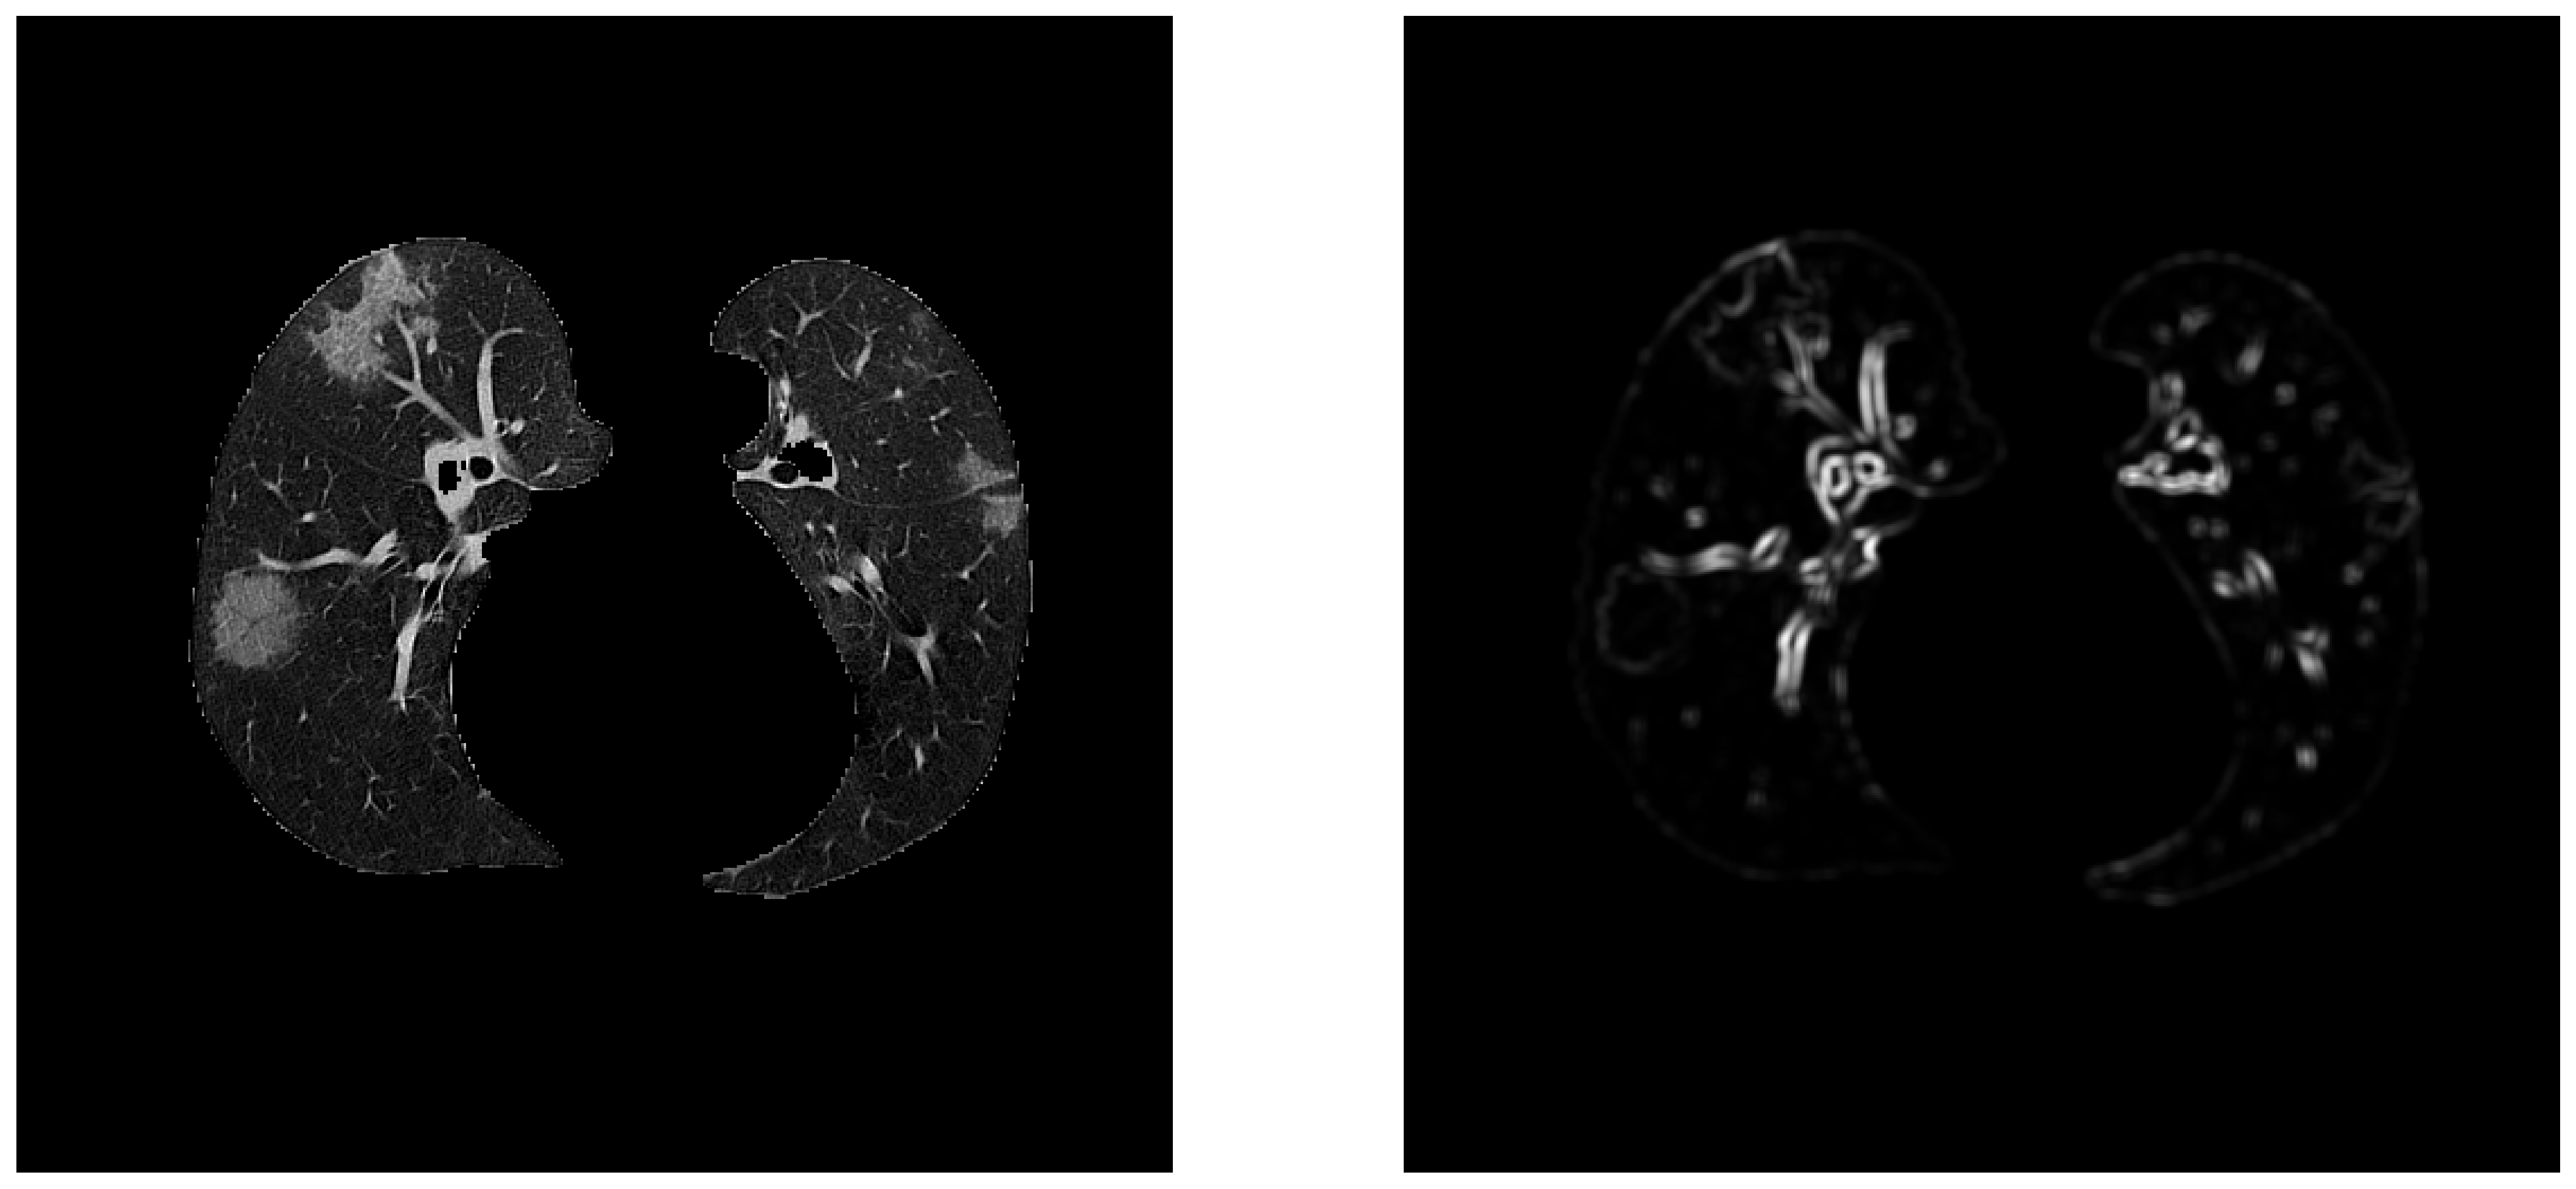
\includegraphics[scale=.3]{MaxEigenVal.png}
		\caption{From left to right: lung regions selected by the U-Net; ,maximum eigenvalues map of the lung. As we can see the U-Net does not exclude the bronchial structure from the lung, on the other hand, the maximum eigenvalues map delineates very well these regions.We have used this map to remove the unwanted bronchial regions.}\label{fig:MaxEigenval}
	\end{figure}
	
	In \figurename\,\ref{fig:MaxEigenval}, I've displayed the image after the lung segmentation by the neural network, and the corresponding eigenvalues map. As we can see the higher values of the map corresponds to the edges of the main bronchial structures. To create the mask for these structures a simple threshold on the map was taken. Since the main bronchial structures are large, this process is able to remove only part of the edges, but the inner structure is preserved. In order to refine the segmentation, this process is repeated a second time, allowing a more accurate exclusion of the structures.
	
	\subsubsection*{Training}
	
	This step involves the estimation of the centroids for each tissue. To achieve this purpose I have chose to perform a clustering using the k-means algorithm. 
	
	I have to takes into account that the k-means clustering requires a balanced representation for each cluster. As we can see in \figurename\,\ref{fig:ClusterRepr}, the main part of the image is composed to background. This cluster is over-represented. Moreover we can observe that the amount of involved lung volume may change according to the  severity of the disease: the first scan presents a low amount pf GGO and CS; se second one have a larger region involves.
	
	To overcome these issue, I have simply removed the background from the segmentation and carefully selected the scans of the training set to ensure an balanced representation of each cluster.

	In summary, the implementation of this step involves the building of the multi-channel image, which allow us to takes into account also the neighborhood information, the managing of the over represented clusters and the actual centroids estimation.
	
	\begin{figure}[h!]
		\centering
			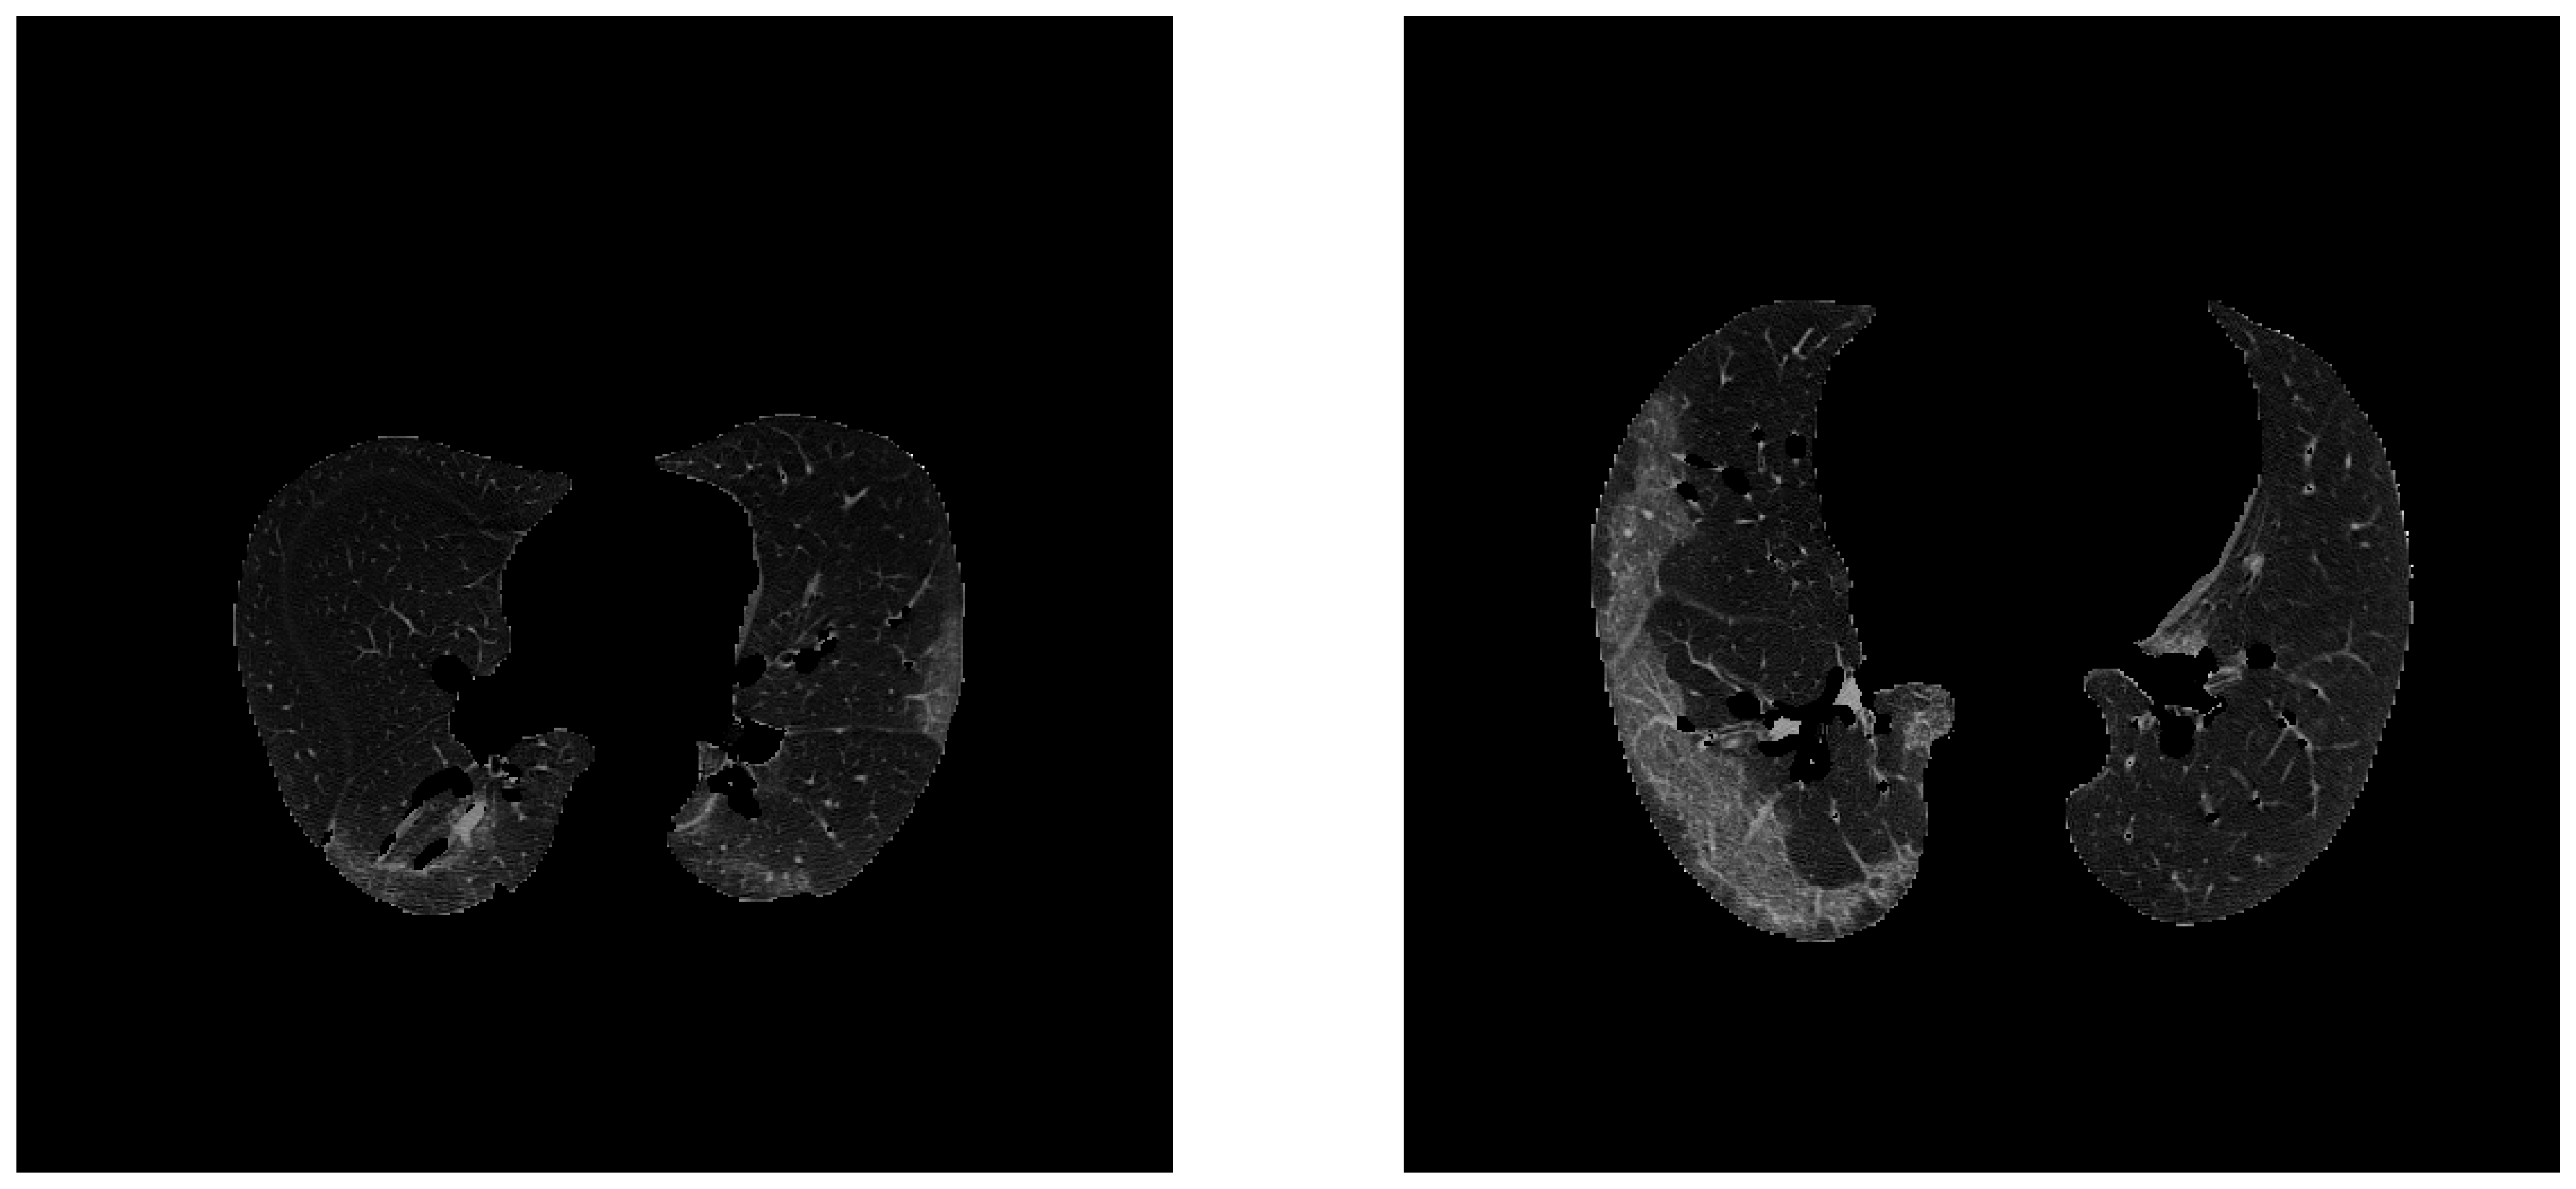
\includegraphics[scale=.4]{ClusterRepr.png}
			\caption{Lung regions with different ground glass areas. We can notice that the main part of the image is composed only by the background. From left to right respectively a scan with small lesion areas and one with a large lesion. }\label{fig:ClusterRepr}
	\end{figure}

	\subsubsection*{Labeling}
	
	This step involves the actual segmentation. The script which perform it requires as inputs the CT scans after the lung extraction, and the previously estimated centroids. This block of the pipeline simply assigns each voxel to the cluster corresponding to the nearest centroids then select the only one corresponding to GGO and CS areas. In this way we are performing a pixel classification by assigning the regions to a particular labels according only to their intensities information: this allow us to group on the same cluster objects that are spatially disconnected as often happen in the medical imaging field.\\
	The distance between voxel colors and each centroid is defined as the euclidean distance:
	\begin{equation*}
		d(x_j, c_i) = \sqrt{(x_j - c_i)^2}
	\end{equation*} 
	Where $x_j$ is the color vector for the $j_{th}$ voxel and $c_i$ is the $i_{th}$ centroid.\\
	

	
\end{document}